%% LaTeX2e class for student theses
%% sections/main/1_fundamentals.tex
%%
%% Karlsruhe University of Applied Sciences
%% Faculty of  Computer Science and Business Information Systems
%%
%% --------------------------------------------------------
%% | Derived from sdqthesis by Erik Burger burger@kit.edu |
%% --------------------------------------------------------


\chapter{Fundamentals}
\label{ch:Fundamentals}

The subsequent chapter provides a fundamental understanding of the concepts and general conditions, which apply in the sector of \gls{emobility}, and therefore are omnipresent in most of the described scenarios later on.
First of all, section \ref{ch:Fundamentals:sec:Electric Mobility} gives a general review of \gls{emobility}, like the involved actors and its systems. Furthermore, existing standards for picturing the communication between these actors and systems and a brief introduction of smart charging including its variations follow.
The next section \ref{ch:Fundamentals:sec:Reservation Systems} illustrates the basic functionality of a reservation system itself, its use cases and a differentiation between common types of reservation systems.
Finally, section \ref{ch:Fundamentals:sec:Data Exchange} lists important communication protocols and data exchange formats used in the according standards described in \ref{ch:Fundamentals:sec:Electric Mobility:ssec:Relevant Standards}.

\section{Electric Mobility}
\label{ch:Fundamentals:sec:Electric Mobility}

The term \Gls{emobility} generally refers to the use of \acrfull{ev} and other electric-powered transportation options as an alternative to conventional vehicles that are powered by an \acrfull{ice}. 
As key component of the global effort to tackle climate change and achieve sustainable transportation solutions, it targets the reduction of greenhouse gas emissions, decrease dependence on fossil fuels, and mitigate the environmental impact of transportation \cite{kathiresh_e-mobility_2022}.
To reach this goal, \Gls{emobility} depends on the expansion of \acrshortpl{ev} as general mean of transportation and a tighter cluster of \acrshortpl{cs}.

\subsection{Electric Vehicles}
\label{ch:Fundamentals:sec:Electric Mobility:Electric Vehicles}

As mentioned in section \ref{ch:Fundamentals:sec:Electric Mobility}, \acrshortpl{ev} are a fundamental cornerstone of \Gls{emobility}. A \acrshort{ev} describes an automobile, which is powered by only one or more electric engines drawing energy from onboard batteries or similar energy sources. 
Beside \acrfullpl{bev}, which are purely powered by electricity, further invariants like \acrfullpl{phev} or \acrfullpl{hev} exist. In comparison to \acrshortpl{bev} a \acrshortpl{phev} combine an electric motor with an internal combustion engine.
This enables the driver to bridge shorter distances by only using the power of the internal battery and rely on the \acrshort{ice} during longer trips and no sufficient charging opportunities. Additionally, \acrshortpl{phev} are capable of recharging the battery while driving.
Therefore, they use the brake resistance to alter the resulting power into electricity, which goes directly into the battery.
\acrshortpl{hev} are very similar to \acrshortpl{phev}, because they could use both power sources. But in contrast to a \acrshort{phev}, a \acrshort{hev} cannot be plugged in for charging \cite{kathiresh_e-mobility_2022}.

\begin{figure}[h]
    \centering
    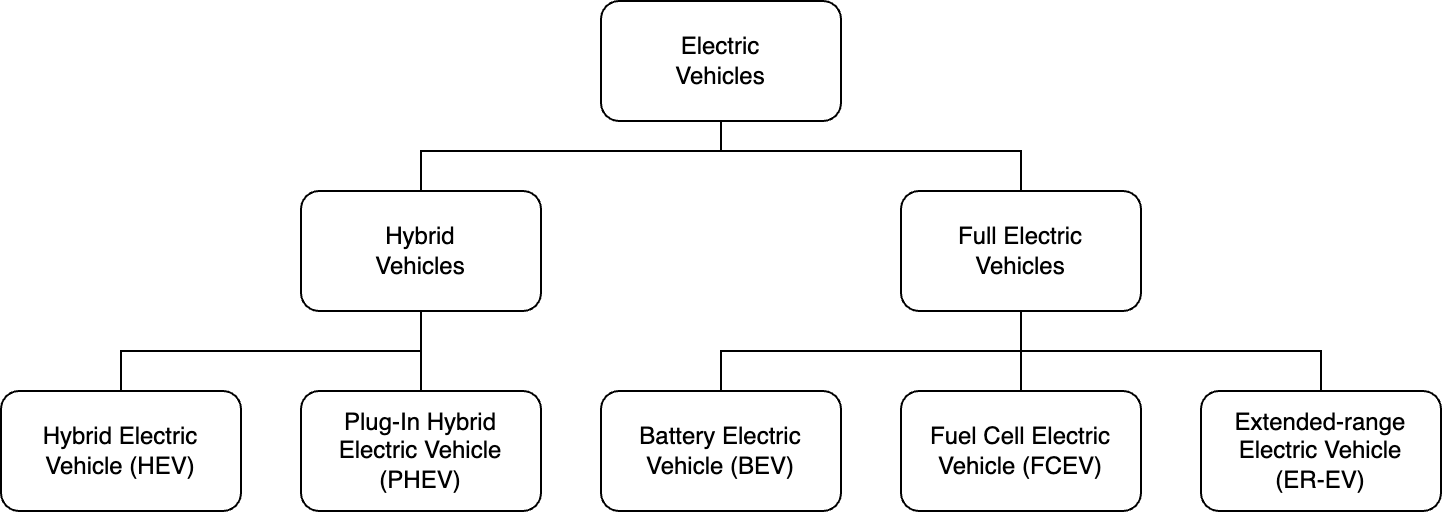
\includegraphics[scale=0.4]{resources/images/main/1_fundamentals/ElectricVehicleTypes.png}
    \caption{Classification approach for different \acrshort{ev} types based on \cite{acharige_review_2023}.}
    \label{fig:ev-classification}
\end{figure}

\subsection{Charging Infrastructure}
\label{ch:Fundamentals:sec:Electric Mobility:ssec:Charging Infrastructure}

To charge the increasing number of \acrshortpl{ev}, a wide spread charging infrastructure composed of \acrshortpl{cs} is a critical component. As mentioned in \cite{gnann_fast_2018}, the charging infrastructure needs are highly depending on the battery sizes and power rates, which are approximately about to increase.
Based on the vehicle and used battery, the power demand is varying. Therefore, the stations and the associated charging levels could range from slow \acrshortpl{cs} with a power offer, which ranges to 22 \acrshort{kW} and fast \acrshortpl{cs} for power demands above this range. \\
\noindent Getting a better understanding of the different scenarios, a \acrshort{cs} could be used for charging, this work divides the infrastructure and the according stations into three different groups. These groups, separated by accessibility to the \acrshortpl{evu}, are listed with the corresponding user limitation, the associated locations and the charger levels mostly used, in the table \ref{tab:cs-accessibility-levels} below:

\begingroup
\setlength{\tabcolsep}{10pt} % Default value: 6pt
\renewcommand{\arraystretch}{1.5} % Default value: 1
\begin{table}[h]
\centering
\caption{Differentiation of accessibility in case of charging opportunities based on \cite{kathiresh_e-mobility_2022},\cite[18-19]{linnemann_elektromobilitat_2020}.}
    \begin{tabular}{c|c|m{5.5cm}|c}
    Accessibility & Restrictions & Location & Charging Level \\ \hline
    Public & No & fleets, highway, distribution centers & 3 \\
    Semi-Public & Yes & workplace, hotels & 2 \\
    Private & Yes & private households & 1 
    \end{tabular}
\label{tab:cs-accessibility-levels}
\end{table}
\endgroup

\noindent Alongside the separation according to the accessibility level, a differentiation based on classes of \acrfullpl{cs} is possible. For illustration of the dependencies and affiliations between the different classes, the following illustration \ref{fig:charging-station-classification} shows a detailed overview. 

\begin{figure}[h]
\centering
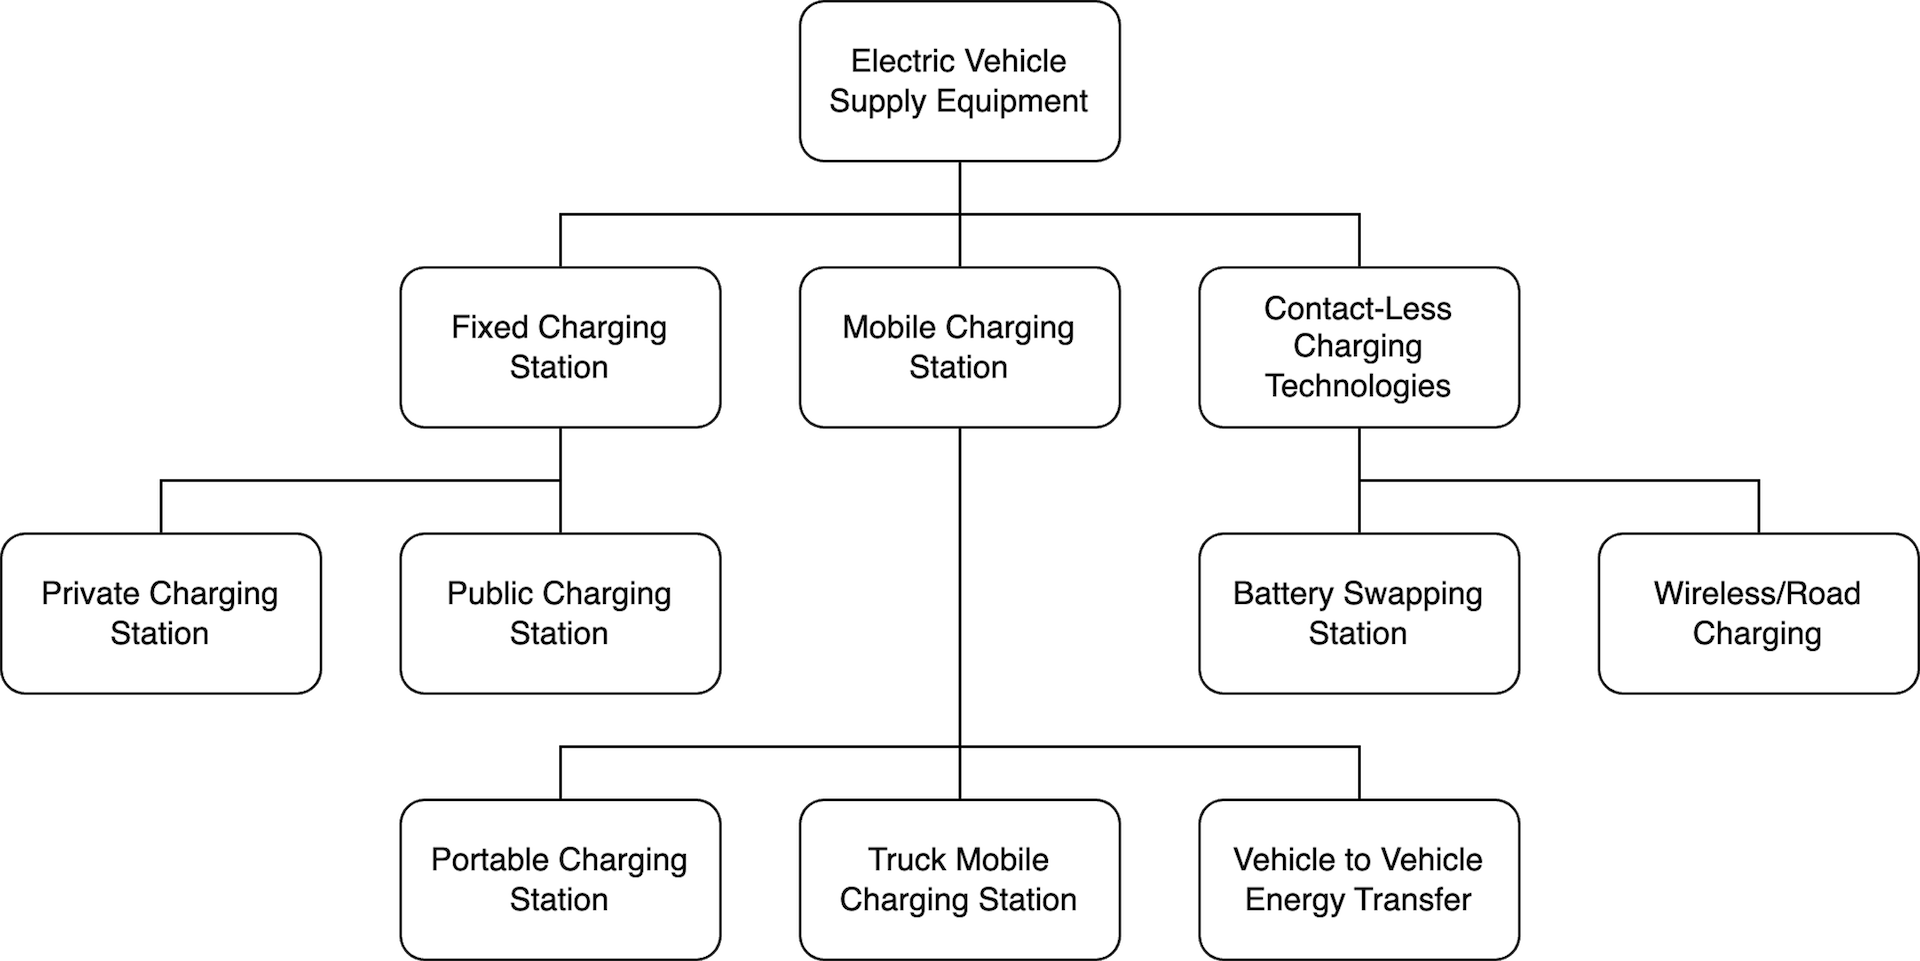
\includegraphics[scale=0.4]{resources/images/main/1_fundamentals/ChargingStationClassification.png}
\caption{Classification for different types of charging stations based on \cite{afshar_literature_2020}.}
\label{fig:charging-station-classification}
\end{figure}

\noindent To provide a more detailed view on the infrastructure and the hardware used for charging, also referred to as \acrfull{evse}, all components and systems necessary to supply electric power from the grid to the battery of an \acrfull{ev} are explained afterwards.
Beginning with the \textbf{\acrfull{cs}} itself, as physical power unit the \acrshort{ev} is connected to. As mentioned above, a \acrshortpl{cs} could vary in size and complexity, ranging from small wall-mounted units designed for home use to more extensive public \acrshortpl{cs} found in parking lots, shopping centers or along highways. 
To establish a connection between grid, \acrshort{cs} and car, a \textbf{Connector or Charging Cable} is needed. It contains plugs on both ends, which are connecting to the vehicle's charging port and to the \acrshortpl{cs} outlet. 
As an integral part of the \acrshort{evse}, the \textbf{\acrshort{pms}} regulates the flow of electricity from the grid to the vehicle's battery. It ensures safe and efficient charging, managing the power level based on the vehicle's battery capacity and the grid's capacity.
Allowing the communication between the \acrshort{ev}, the \acrfull{cs} and the grid, a \textbf{\acrshort{cms}} as a backend is used. It allows data exchange regarding charging status, electricity prices, user authentication, and other relevant information.
In case of public \acrshortpl{cs}, a payment and authentication system is usually integrated into the \acrshort{evse}. This system verifies the user's identity, authorizes the charging session, and processes payment for the electricity consumed.
On top of the described components, various safety features are integrated to protect users, the vehicle, and the surrounding environment. This includes features like ground fault protection, over-current protection, temperature monitoring, and emergency shut-off capabilities \cite{littlefuse_designing_2020}.

\noindent To cover the wide range of existing \acrshortpl{ev} and their individual power demands, different categories of chargers based on the provided power level were established. In the context of this work, the most prominent ones are listed in \ref{tab:ev-charging-levels} with a high-level overview about their specifications and their usual application. 

\begingroup
\setlength{\tabcolsep}{10pt} % Default value: 6pt
\renewcommand{\arraystretch}{1.5} % Default value: 1
\begin{table}[h]
    \centering
    \caption{Listing of different \acrshort{ev} charging levels based on \cite{acharige_review_2023}.}
    \begin{tabular}{c|c|m{6.5cm}}
        Charging Level & Charging Power & Use Case \\ \hline
         1 & 1.44 \acrshort{kW} - 1.9 \acrshort{kW} & Typically the slowest charging option and suitable for overnight charging at home \\
         2 & 3.1 \acrshort{kW} - 19.2 \acrshort{kW} & Provides faster charging compared to Level 1 and is commonly used for home charging setups and public charging stations \\
         3 & 20 \acrshort{kW} - 350 \acrshort{kW} & Fast charging operates at a higher voltage, directly charging the vehicle's battery with \acrshort{dc} power. Commonly used in public fast-charging stations.\\
         \acrshort{xfc} & > 350 \acrshort{kW} & Ultra-fast charging provides the fastest charging option. Commonly used in commercial settings.
    \end{tabular}
    \label{tab:ev-charging-levels}
\end{table}
\endgroup

\newpage

\subsection{Battery Technology}
\label{ch:Fundamentals:sec:Electric Mobility:ssec:Battery Technology}

For storing the required energy, \acrshortpl{ev} rely on their build-in batteries. As key components inside an \acrshort{ev}, they have to handle high energy capacity and high power within limited weight and space to affordable prices.
Therefore, most manufacturers use Lithium-ion batteries in their cars nowadays. 
Alternatives like \textit{Lead Acid} and \textit{Nickel-based} batteries lack in comparison to lithium-based batteries mostly in shorter life cycles, insufficient performance in extreme climate conditions or higher discharging rates \cite{acharige_review_2023}.
Generally, further advancements in this technology like the increase in range of \acrshortpl{ev} and the reduction of charging duration in combination with cost-effectiveness are an essential part of the turnover from cars with \acrshort{ice} to \acrshort{ev}.

\subsection{Relevant Standards}
\label{ch:Fundamentals:sec:Electric Mobility:ssec:Relevant Standards}

To provide a general interface for information exchange between \acrshortpl{cs}, \acrshortpl{ev} and their users, several organizations, initiatives and the industry established several standards.
Beside the \acrfull{ocpp} \cite{noauthor_ocpp_nodate}, a communication protocol, developed by the \acrfull{oca} \cite{noauthor_open_nodate}, other protocols and specifications exist, covering different aspects and scenarios relevant during or before the charging process.
In addition to the previous mentioned \acrshort{ocpp}, further standards relevant in this work will be listed and explained afterwards.

\subsubsection{Open Charge Point Protocol}
\label{ch:Fundamentals:sec:Electric Mobility:ssec:Relevant Standards:sssec:OCPP}

The \acrfull{ocpp} describes an open industry-standard communication protocol used especially in charging infrastructure for \acrshortpl{ev}. Proposed by the ElaadNL foundation as an open protocol supporting the communication between \acrshort{cs} and the corresponding backend services, resulting in a transfer of ownership to \acrshort{oca} in 2014 \cite{garofalaki_electric_2022}.
In general, the \acrshort{ocpp} is designed to provide interoperability and seamless integration between different charging station vendors and network operators, ensuring that \acrshort{ev} drivers can charge their vehicles at any compatible \acrshort{cs}. 
Therefore, it is maintained by the \acrfull{oca}, a consortium of \acrshort{ev} charging infrastructure stakeholders, as open protocol and not proprietary to any specific manufacturer or organization. 
This should ensure that the \acrshort{ocpp} remains a collaborative and evolving standard \cite{noauthor_ocpp_nodate}. \\
From an architectural point of view, the protocol could be described in form of a client/server architecture. The \acrshort{evse} in this model acts as the client, while the \acrshort{csms} serves as the server. 
The server responds to the client's requests and manages the charging processes accordingly. This request-response model, where the client sends requests to the server, and the server responds with the appropriate information or action enables real-time communication between the \acrfull{cs} and the connected \acrfull{cms}.
As an interface for communication, two different types of protocols are used. On the one side, the WebSocket protocol, described in \ref{ch:Fundamentals:sec:Data Exchange:ssec:WebSocket}, for bidirectional communication, providing a persistent connection between the \acrshort{evse} and the \acrshort{cms} and allowing a faster and more efficient data exchange. On the other side, \acrfull{soap}, see \ref{ch:Fundamentals:sec:Data Exchange:ssec:SOAP}, could be used for one-way communication.
To differentiate between particular feature sets, the \acrshort{ocpp} is versioned. 
The versions are illustrated as floating point numbers, which are increasing based on major or minor releases. 
The most recent protocol versions, often used in existing applications, are \acrshort{ocpp} 1.6 and \acrshort{ocpp} 2.0. \\ \\
\noindent For the communication between \acrshort{cs}, \acrshort{csms} and the \acrshort{evu} the \acrshort{ocpp} protocol relies on so called operations. Each of these operations describes a set of instructions, which are necessary to fulfill, to successfully complete the underlying process.
According to the required operations used in the context of this work, a subset of operations are selected, which are elucidated in the following list. 
The wording and the explanations are based on the standard documentation for the \acrshort{ocpp} version 1.6 \cite{noauthor_ocpp_nodate}:

\begin{description}
    \item[Authorize] Before starting a charging session, the \acrshort{evu} \acrfull{rfid} card or other identification is sent to the central system for authorization. The \acrshort{cms} checks the driver's credentials and responds with an authorization status.
    \item[Start Transaction] After successful authorization, the \acrshort{cms} sends a start transaction request to initiate the charging process. The \acrshort{cs} acknowledges the request, and the charging session begins.
    \item[Status Notification] The \acrshort{cs} may send status notifications to the \acrshort{cms} to update the current state of the \acrshort{cs}, such as \verb|Available|, \verb|Charging|, \verb|Reserved|, or \verb|Faulted|.
    \item[Reserve Now] In case a user needs an available connector on a \acrshort{cs}, he could send a \textbf{Reserve Now} request via the \acrshort{cms} to the \acrshort{cs}, which reserves one specific or at least on connector on the station for a specified duration. The according connector in case of successful reservation changes from status \verb|Available| to \verb|Reserved|.
    As a result, only the user assigned to the deposited \acrshort{rfid} card is able to start charging at the specified connector or the superior \acrshort{cs}.
    \item[Cancel Reservation] For cancelling the created reservation the user could manually send a request with the assigned reservation id to the \acrshort{cms} to free the connector again. Otherwise, the \acrshort{cs} will notify the \acrshort{cms}, if the reservation reaches its expiry limit.
\end{description}

\subsubsection{Open Charge Point Interface}
\label{ch:Fundamentals:sec:Electric Mobility:ssec:Relevant Standards:sssec:OCPI}

\acrfull{ocpi} is an open standard for communication designed interoperability among various charging network operators, enabling \acrshort{ev} drivers to access charging infrastructure from different providers using a unified and standardized approach. 
Aside \acrshort{ocpi}, other approaches regarding the developement of cross-border EV travel, also known as 'e-roaming', exist. 
The most prominent ones are \acrfull{oicp}, \acrfull{ochp} and \acrfull{emip} \cite{ferwerda_advancing_2018}. 
In contrast to the \acrshort{ocpi}, they are all developed by proprietary institutions and integrated inside their roaming platforms.
This makes the \acrshort{ocpi} standard more suitable in case of an openness and interoperability. \\
\noindent In case of available features, \acrshort{ocpi} provides defined endpoints, used for communication between \acrshort{cs}, \acrshortpl{cms}, \acrshortpl{emsp} and \acrshortpl{cpo}. These endpoints include for example functionalities like location discovery, charge point data, authorization, charging sessions, and error handling. 
For integrating \acrshort{ocpi} into existing software systems it is heavily based on the paradigm of \acrfull{rest}. This allows communication via standard HTTP methods utilizing \acrfull{json} as data format for transmitting information. 

The listing below provides a short overview of available features and functionalities provided by \acrshort{ocpi} \cite{noauthor_open_2021}:

\begin{description}
    \item[Location Discovery] Charging networks can exchange information about available charging locations, providing details such as location coordinates, \acrshort{cs} types, and status.
    \item[Charge Point Data] \acrshort{cs} data, including information on \acrshort{cs} availability, status, and pricing, can be accessed through \acrshort{ocpi}.
    \item[Charging Sessions] \acrshort{ocpi} supports real-time information about ongoing charging sessions, including start time, energy consumed, and current charging status.
    \item[Authorization and Authentication] In combination with their respective \acrshort{cpo} accounts or other authentication methods \acrshortpl{evu} are able to be authenticate themselves to access charging services.
    \item[Remote Start/Stop Charging Sessions] To initiate charging sessions, \acrshortpl{evu} could remote start and stop their current charging sessions. This allows the driver to initiate charging sessions via their mobile apps or other remote means.
    \item[Tariff Information] Charging networks can share pricing and tariff information, providing transparency to \acrshortpl{evu} about the cost of charging at different locations.
\end{description}

\subsubsection{ISO 15118}
\label{ch:Fundamentals:sec:Electric Mobility:ssec:Relevant Standards:sssec:ISO 15118}

To address the needs of \acrshortpl{evu} and countering the problems of missing standardization in interoperability of charging infrastructure and information exchange between grid \acrshort{evse}, \acrshort{ev} and \acrshort{evu} Daimler and RWE started in September 2009 with a collaboration to enable Smart Charge Communication.
Until its first release as standard for Plug-and-Charge connections in June 2014, further development according a standardization of charging infrastructure communication was done \cite{heinrich_iso_2017}.
Nowadays, this standard consists out of multiple parts. Beginning with the analysis of the underlying use cases to description of requirements for the communication over the different \acrshort{osi} layers \cite{brosi_methode_2019}.
Furthermore, it describes \acrshort{poi}-data, the \acrshort{cs} availability, payment, communication standards as well as 'Plug \& Charge' ('e-Roaming'). However, the required granularity or level of quality of the data are not specified \cite{linnemann_elektromobilitat_2020}.
In respect of these gaps, still existing in the \acrshort{iso} 15118, it is far away from completeness and requires further development and adjustments.

\subsection{Smart Charging}
\label{ch:Fundamentals:sec:Electric Mobility:ssec:Smart Charging}

The technology of smart charging or intelligent charging, is a systematic approach, which optimizes the charging process of  \acrshortpl{ev} to be more efficient, cost-effective, and environmentally friendly utilizing information and communication technologies, considering factors such as electricity demand, grid capacity, renewable energy availability, and preferences of single users \cite{deb_smart_2022}.
One of the primary goals of this methodology is to balance the demand on the underlying grid, affected by charging large numbers of \acrshortpl{ev} simultaneously \cite{daina_electric_2017}. Especially during peak hours increased electricity costs or potential blackouts could result. 
Therefore, smart charging takes the current load of the grid into account and adjust the possible charging rates based on the given constraints to prevent overloading the grid and optimizing the use of available energy \cite{garcia-villalobos_plug-electric_2014}. 
Beside the unidirectional charging method originally called \acrfull{v1g}, the approach of \acrfull{v2g} enables smart charging systems to charge bidirectionally between the \acrshortpl{ev} battery and the grid \cite[199]{kathiresh_e-mobility_2022}. During times of high demand, \acrshortpl{ev} with sufficient battery capacity can supply energy to the grid. This concept turns \acrshortpl{ev} into mobile energy storage units, enhancing grid stability and resiliency.
To offer all these functions, smart charging relies on data connectivity and communication between the single \acrshortpl{cs}, the \acrshortpl{ev} and the underlying grid, which makes it vulnerable for malign third-party entities as well. On the other side, these aspects are capable of contributing to an overall improved grid management. Grid operators could gain insights into electricity demand patterns and plan grid upgrades accordingly.

\subsection{Smart Grid}
\label{ch:Fundamentals:sec:Electric Mobility:ssec:Smart Grid}

In general, the terminology of a \acrfull{sg} describes the characteristics of an intelligent system dealing with high energy consumption in order to increase the energy reliability and the corresponding costs \cite{sharma_smart_2020,moreno_escobar_comprehensive_2021}.
It consists of multiple parts, like a sufficient infrastructure, applications and several technologies to manage the energy flow inside the grid.
For example monitoring and measuring solutions are important example for technologies, allowing the grid to support an efficient generation and distribution of power. Additionally, the behaviour of the users connected to the \acrshort{sg}, are part of the optimization processes taking place inside.
These processes are part of algorithms implemented by an central orchestration system, which observes the \acrshort{sg}.
Based on \cite{moreno_escobar_comprehensive_2021} till now, 94 possible algorithms for optimization are known, to manage these kind of networks in an efficient manner.
As a result, the smart grid could control, based on the objectives, the power flow dynamically and in an intelligent way to meat the demands of all the nodes in such a network. 
Compared to the existing grid, which provides power in an unidirectional manner, smart grids allow the delivering of power in a bidirectional way. Therefore, the smart grid uses so called \acrshort{der}, like \acrshortpl{ev} or renewable energy sources at consumer homes, making their power available, if they do not need them.
This approach is very similar to the \acrshort{v2g} functionality of smart charging described in \ref{ch:Fundamentals:sec:Electric Mobility:ssec:Smart Charging} and could be combined.


\section{Reservation Systems}
\label{ch:Fundamentals:sec:Reservation Systems}

Originally developed in form of a \acrfull{crs} as part of a collaboration between airline and technology companies \cite{xiang_evolution_2020}, reservation systems main objective as tool for booking resources without the need of paper or other systems for organization, evolved over the time.
Started as a centrally managed system with restricted access to call center operators, which administered the available resources for their corresponding airlines or hotel chains, the further development of the world wide web in 1989 led to a transformation away from the \acrshort{crs} to online booking systems, also known as web-based \acrfullpl{ibe}, directly available to the customer via their personal computers at home.
In general, a reservation system could be described by definition as a software application or platform that facilitates the process of booking and securing limited services, resources, or accommodations in advance. 
As mentioned above, beside its original usage in travel or hospitality, it is a common tool for administration in transportation or entertainment industries. 
Leading to streamlined reservation processes for customers or clients, which allow the reduction of administrative workload and enhance the users experience.
Based on the system architecture and used technologies, reservation systems could differ in case of needed functionalities. Used as part of a web-based application like the online booking system, different constraints and use cases have to be taken into account as in case of a local system inside one institution. 
To abstract from the requirements needed for specific deployment scenarios, the following part describe a set of key features and functionalities a reservation system typically should include. The list of selected features may not cover each use cases needed for a specific system, but should provide a brief overview in case of a general purposes.
As a reference and guiding principle in case of reservation system functionality, existing research and literature on hotel reservation systems like \cite{delizo_online_2013, bemile_online_nodate} is used.
\textbf{Booking and Scheduling (i)} could be described as main purpose of a reservation system. By using this feature users can view available dates, times, or slots and make reservations for specific services, activities, or resources. The system ensures that conflicting bookings do not occur.
To provide an overview, which represents the availability of the above specified resource, the system requires \textbf{Real-Time Availability (ii)}. Therefore, Users can see immediately if the desired service or resource is available for the chosen date and time.
For personalization of the user experience, the possibility to store a reservation history and in regards of loyalty rewards, a \textbf{User Registration and Authentication (iii)} for creating an account or logging into the system for creating reservations should be provided.
Furthermore, a possibility to pay for the users booking by a secure payment processing using credit card or digital wallets in form of \textbf{Online Payments} is often included in these kind of systems.
To acknowledge successful reservations or notify the user in case of changes to its reservation, \textbf{Confirmation and Notifications (iv)} should be integrated into the system. Beside the function as confirmation of the booking, it serves as proof for the reservation and could include details like booking ID, date, time and location.
Regarding the need of modification or cancellation of the reservation, the system should provide \textbf{Cancellation and Modification (v)} features, enable the user to cancel or modify their reservations within a specified time frame. Additionally  cancellation policies could be used for penalties in case of late cancellations.
Alongside the management of the reservations made via the system, it should provide a \textbf{Inventory Management (vi)} for the owners of the provided resources and helping them to manage their possessions.
% TODO: Redefinition
Tools for \textbf{Reporting and analytics (vii)} or \textbf{Integration with Other Systems (viii)} for generating reports on booking trends, revenue, occupancy rates or integrate with other software or systems, such as customer relationship management (CRM) software, payment gateways could be integrated.

\section{Data Exchange}
\label{ch:Fundamentals:sec:Data Exchange}

After the introduction of the different services and their communication channels and provided information in section \ref{ch:Fundamentals:sec:Electric Mobility:ssec:Relevant Standards}. The following section describes the underlying technical concepts integrated into the used protocols.
Beside a short overview of \acrfull{rest} in \ref{ch:Fundamentals:sec:Data Exchange:ssec:REST}, a brief summary of the technologies \acrfull{soap} in \ref{ch:Fundamentals:sec:Data Exchange:ssec:SOAP} and WebSockets in \ref{ch:Fundamentals:sec:Data Exchange:ssec:WebSocket} follow. 

\subsection{REST}
\label{ch:Fundamentals:sec:Data Exchange:ssec:REST}

Introduced as an architectural style by Roy Fieldings \cite{patni_pro_2017} for designing distributed systems, \acrfull{rest} provides concepts and a set of constraints defining resources accessed via a common interface by \acrshort{http} standard methods.
The most common \acrshort{http} methods for querying a \acrshort{rest} \acrshort{api} are \verb|GET|, \verb|POST|, \verb|PUT| and \verb|DELETE| and representing CRUD operations similar to the operations used in the context of relational and non-relational databases.
To define conceptual targets, \acrshort{rest} defines so called resources, which are mapped by resource identifiers in the form of a uniform resource locator (URI) or a uniform resource name (URN). Using this pattern a valid resource representing a list of cars could be described in the form of \verb|http://rest.service.com/cars|. 
Sending a \acrshort{http} request with  \verb|GET| method to this resource, a list of cars should be returned.
The representation of the returned data could be in the form of \acrshort{json} or whole \acrshort{html} documents and even images are allowed.
Further data elements defined by \acrshort{rest} are resource metadata, representation metadata and control data, which are only mentioned here for completeness. 
Beside this fundamental elements, \acrshort{rest} offers a wide range of variations regarding application and system design but are not necessary in the context of this work.

\subsection{SOAP}
\label{ch:Fundamentals:sec:Data Exchange:ssec:SOAP}

As counterpart to the \acrshort{rest} described in the previous section \ref{ch:Fundamentals:sec:Data Exchange:ssec:REST}, \acrshort{soap}, created by Dave Winer and others in corporation with the company Microsoft \cite{patni_pro_2017}, addresses the needs of enterprise software.
The basic concept behind \acrshort{soap} is offering of data in form of services, which are labeled using names consisting out of verbs and nouns. For example the service called \textit{getCar} should provide information about cars and does not fulfill any other purpose.
In contrast to \acrshort{rest}, information about the handled objects is communicated to the client and could be described with a \acrshort{wsdl}.
This ensures a so called contract between a server and a client, which provides beside security and authorization direct access to objects available on the server.
As mentioned in \cite[4]{patni_pro_2017}, \acrshort{soap} should be used, when the use case handling transactional operations or the environment requests this protocol.

\subsection{WebSocket}
\label{ch:Fundamentals:sec:Data Exchange:ssec:WebSocket}

Based on the RFC 6455 \cite{melnikov_websocket_2011}, the WebSocket protocol enables a two-way communication between a client and a remote host. After establishing trust via the origin-based security model commonly used by today's browsers. After initiating the connection and trust establishment, the protocol communicates via basic message framing, layered over \acrshort{tcp}.
This allows applications, basically developed for usage in the web, a creation of a two-way communication with servers without relying on opening multiple HTTP connections.
Beside the usage over unencrypted HTTP channels, the WebSocket protocol could utilize encrypted traffic via HTTPS on port 443.
